%----------------------------------------------------------------------------------------
%	PACKAGES AND OTHER DOCUMENT CONFIGURATIONS
%----------------------------------------------------------------------------------------

\documentclass{article}

\usepackage{fancyhdr} % Required for custom headers
\usepackage{lastpage} % Required to determine the last page for the footer
\usepackage{extramarks} % Required for headers and footers
\usepackage[usenames,dvipsnames]{color} % Required for custom colors
\usepackage{graphicx} % Required to insert images
\usepackage{listings} % Required for insertion of code
\usepackage{courier} % Required for the courier font
\usepackage{lipsum} % Used for inserting dummy 'Lorem ipsum' text into the template
%Math related packages
\usepackage{amsmath}
\usepackage{amssymb}
%Recurrence Tree
\usepackage{tikz}
\tikzstyle{vertex}=[draw,fill=black!15,circle,minimum size=20pt,inner sep=0pt]

% Margins
\topmargin=-0.45in
\evensidemargin=0in
\oddsidemargin=0in
\textwidth=6.5in
\textheight=9.0in
\headsep=0.25in

\linespread{1.1} % Line spacing

% Set up the header and footer
\pagestyle{fancy}
\lhead{\hmwkAuthorName} % Top left header
\chead{\hmwkClass\ (\hmwkClassInstructor\ \hmwkClassTime): \hmwkTitle} % Top center head
\rhead{\firstxmark} % Top right header
\lfoot{\lastxmark} % Bottom left footer
\cfoot{} % Bottom center footer
\rfoot{Page\ \thepage\ of\ \protect\pageref{LastPage}} % Bottom right footer
\renewcommand\headrulewidth{0.4pt} % Size of the header rule
\renewcommand\footrulewidth{0.4pt} % Size of the footer rule

\setlength\parindent{0pt} % Removes all indentation from paragraphs
%----------------------------------------------------------------------------------------
%    Code Snippet
%   
%----------------------------------------------------------------------------------------
\usepackage{listings}
\usepackage{color}

\definecolor{dkgreen}{rgb}{0,0.6,0}
\definecolor{gray}{rgb}{0.5,0.5,0.5}
\definecolor{mauve}{rgb}{0.58,0,0.82}

\lstset{frame=tb,
  language=Java,
  aboveskip=3mm,
  belowskip=3mm,
  showstringspaces=false,
  columns=flexible,
  basicstyle={\small\ttfamily},
  numbers=none,
  numberstyle=\tiny\color{gray},
  keywordstyle=\color{blue},
  commentstyle=\color{dkgreen},
  stringstyle=\color{mauve},
  breaklines=true,
  breakatwhitespace=true,
  tabsize=3
}
%----------------------------------------------------------------------------------------
%	DOCUMENT STRUCTURE COMMANDS
%	Skip this unless you know what you're doing
%----------------------------------------------------------------------------------------

% Header and footer for when a page split occurs within a problem environment
\newcommand{\enterProblemHeader}[1]{
\nobreak\extramarks{#1}{#1 continued on next page\ldots}\nobreak
\nobreak\extramarks{#1 (continued)}{#1 continued on next page\ldots}\nobreak
}

% Header and footer for when a page split occurs between problem environments
\newcommand{\exitProblemHeader}[1]{
\nobreak\extramarks{#1 (continued)}{#1 continued on next page\ldots}\nobreak
\nobreak\extramarks{#1}{}\nobreak
}

\setcounter{secnumdepth}{0} % Removes default section numbers
\newcounter{homeworkProblemCounter} % Creates a counter to keep track of the number of problems

\newcommand{\homeworkProblemName}{}
\newenvironment{homeworkProblem}[1][Problem \arabic{homeworkProblemCounter}]{ % Makes a new environment called homeworkProblem which takes 1 argument (custom name) but the default is "Problem #"
\stepcounter{homeworkProblemCounter} % Increase counter for number of problems
\renewcommand{\homeworkProblemName}{#1} % Assign \homeworkProblemName the name of the problem
\section{\homeworkProblemName} % Make a section in the document with the custom problem count
\enterProblemHeader{\homeworkProblemName} % Header and footer within the environment
}{
\exitProblemHeader{\homeworkProblemName} % Header and footer after the environment
}

\newcommand{\problemAnswer}[1]{ % Defines the problem answer command with the content as the only argument
\noindent\framebox[\columnwidth][c]{\begin{minipage}{0.98\columnwidth}#1\end{minipage}} % Makes the box around the problem answer and puts the content inside
}

\newcommand{\homeworkSectionName}{}
\newenvironment{homeworkSection}[1]{ % New environment for sections within homework problems, takes 1 argument - the name of the section
\renewcommand{\homeworkSectionName}{#1} % Assign \homeworkSectionName to the name of the section from the environment argument
\subsection{\homeworkSectionName} % Make a subsection with the custom name of the subsection
\enterProblemHeader{\homeworkProblemName\ [\homeworkSectionName]} % Header and footer within the environment
}{
\enterProblemHeader{\homeworkProblemName} % Header and footer after the environment
}

%----------------------------------------------------------------------------------------
%	NAME AND CLASS SECTION
%----------------------------------------------------------------------------------------

\newcommand{\hmwkTitle}{Assignment\ \#4} % Assignment title
\newcommand{\hmwkDueDate}{,\ Wednesday \ 7,\ 2018} % Due date
\newcommand{\hmwkClass}{CS\ 5800} % Course/class
\newcommand{\hmwkClassTime}{} % Class/lecture time
\newcommand{\hmwkClassInstructor}{Prof. Will Clinger} % Teacher/lecturer
\newcommand{\hmwkAuthorName}{Durwasa Chakraborty} % Your name

%----------------------------------------------------------------------------------------
%	TITLE PAGE
%----------------------------------------------------------------------------------------

\title{
\vspace{2in}
\textmd{\textbf{\hmwkClass:\ \hmwkTitle}}\\
\normalsize\vspace{0.1in}\small{Due\ on\ \hmwkDueDate}\\
\vspace{0.1in}\large{\textit{\hmwkClassInstructor\ \hmwkClassTime}}
\vspace{3in}
}

\author{\textbf{\hmwkAuthorName}}
\date{} % Insert date here if you want it to appear below your name

%----------------------------------------------------------------------------------------

\begin{document}

\maketitle

%----------------------------------------------------------------------------------------
%	TABLE OF CONTENTS
%----------------------------------------------------------------------------------------

%\setcounter{tocdepth}{1} % Uncomment this line if you don't want subsections listed in the ToC

\newpage
\tableofcontents
\newpage

%----------------------------------------------------------------------------------------
%	PROBLEM 1
%----------------------------------------------------------------------------------------

% To have just one problem per page, simply put a \clearpage after each problem

\begin{homeworkProblem}
A)
\begin{figure}[ht]
  \centering\footnotesize
  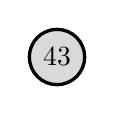
\begin{tikzpicture}[very thick,level/.style={sibling distance=60mm/#1}]
    \node [vertex] (r){$43$};

  \end{tikzpicture}
\end{figure}
\begin{figure}[h]
  \centering\footnotesize
  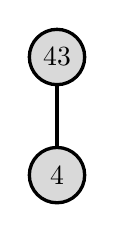
\begin{tikzpicture}[very thick,level/.style={sibling distance=60mm/#1}]
    \node [vertex] (r){$43$}{
    child {node [vertex] (a) {$4$}}
  };

  \end{tikzpicture}
\end{figure}
\begin{figure}[ht]
  \centering\footnotesize
  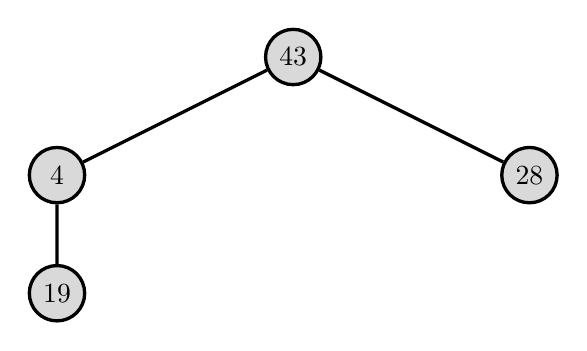
\begin{tikzpicture}[very thick,level/.style={sibling distance=60mm/#1}]
    \node [vertex] (r){$43$}
    child {node [vertex] (a) {$4$}
    		child {
     			 node [vertex] {$19$}
    		}}
    child {node [vertex] {$28$}};

  \end{tikzpicture}
\end{figure}
\begin{figure}[ht]
  \centering\footnotesize
  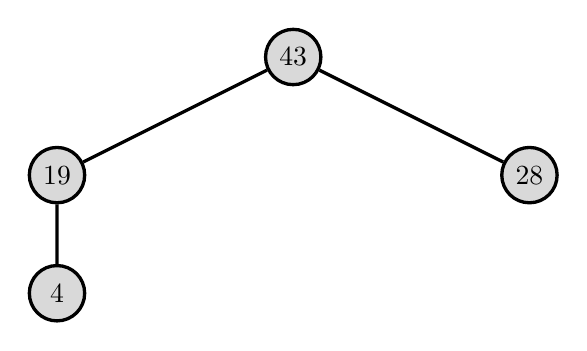
\begin{tikzpicture}[very thick,level/.style={sibling distance=60mm/#1}]
    \node [vertex] (r){$43$}
    child {node [vertex] (a) {$19$}
    		child {
     			 node [vertex] {$4$}
    		}}
    child {node [vertex] {$28$}};

  \end{tikzpicture}
\end{figure}
\begin{figure}[ht]
  \centering\footnotesize
  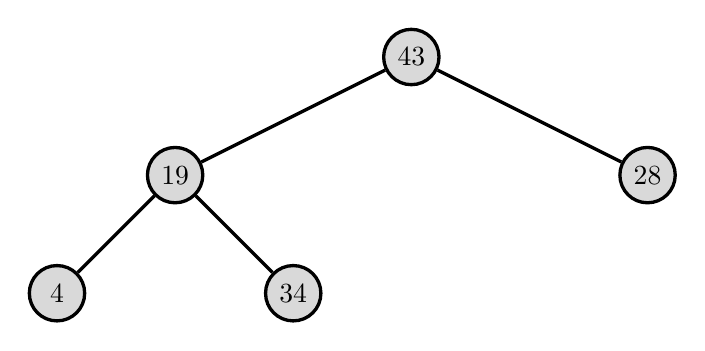
\begin{tikzpicture}[very thick,level/.style={sibling distance=60mm/#1}]
    \node [vertex] (r){$43$}
    child {node [vertex] (a) {$19$}
    		child {
     			 node [vertex] {$4$}
    		}
            child {
     			 node [vertex] {$34$}
    		}}
    child {node [vertex] {$28$}};

  \end{tikzpicture}
\end{figure}
\begin{figure}[ht]
  \centering\footnotesize
  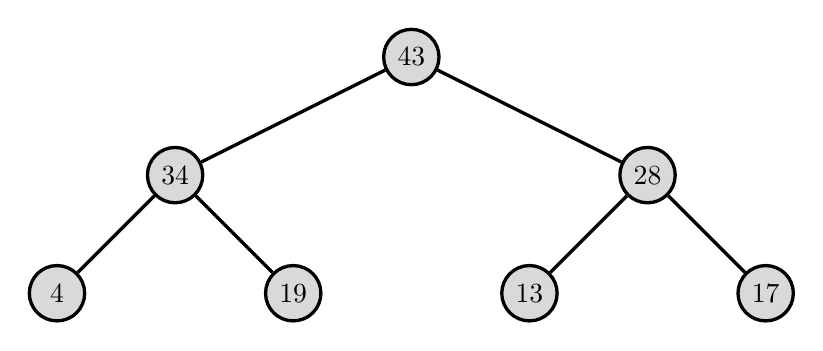
\begin{tikzpicture}[very thick,level/.style={sibling distance=60mm/#1}]
    \node [vertex] (r){$43$}
    child {node [vertex] (a) {$34$}
    		child {
     			 node [vertex] {$4$}
    		}
            child {
     			 node [vertex] {$19$}
    		}}
    child {node [vertex] {$28$}
    		child {
     			 node [vertex] {$13$}
    		}
            child {
     			 node [vertex] {$17$}
    		}};

  \end{tikzpicture}
\end{figure}
\begin{figure}[ht]
  \centering\footnotesize
  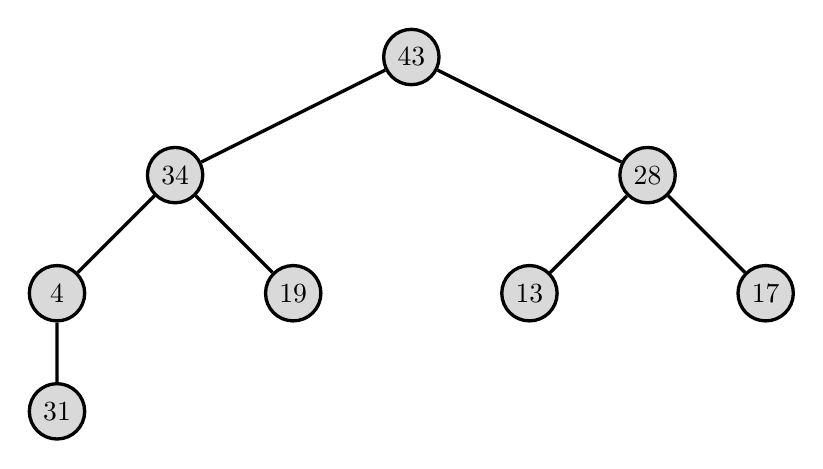
\begin{tikzpicture}[very thick,level/.style={sibling distance=60mm/#1}]
    \node [vertex] (r){$43$}
    child {node [vertex] (a) {$34$}
    		child {
     			 node [vertex] {$4$}
                 	child {
                    	node [vertex] {$31$}
                    }
    		}
            child {
     			 node [vertex] {$19$}
    		}}
    child {node [vertex] {$28$}
    		child {
            	node[vertex] {$13$}
            }
            child {
            	node [vertex] {$17$}
            }};

  \end{tikzpicture}
\end{figure}
\begin{figure}[ht]
  \centering\footnotesize
  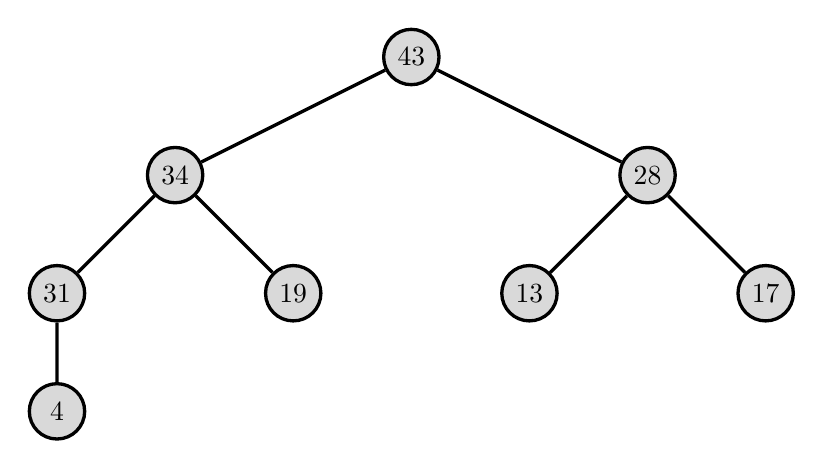
\begin{tikzpicture}[very thick,level/.style={sibling distance=60mm/#1}]
    \node [vertex] (r){$43$}
    child {node [vertex] (a) {$34$}
    		child {
     			 node [vertex] {$31$}
                 	child {
                    	node [vertex] {$4$}
                    }
    		}
            child {
     			 node [vertex] {$19$}
    		}}
    child {node [vertex] {$28$}
    		child {
            	node[vertex] {$13$}
            }
            child {
            	node [vertex] {$17$}
            }};

  \end{tikzpicture}
\end{figure}
\clearpage
\textbf{B)}\\
\\
\begin{figure}[ht]
  \centering\footnotesize
  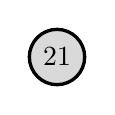
\begin{tikzpicture}[very thick,level/.style={sibling distance=60mm/#1}]
    \node [vertex] (r){$21$};

  \end{tikzpicture}
\end{figure}
\begin{figure}[h]
  \centering\footnotesize
  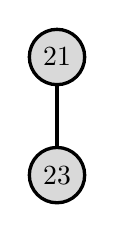
\begin{tikzpicture}[very thick,level/.style={sibling distance=60mm/#1}]
    \node [vertex] (r){$21$}{
    child {node [vertex] (a) {$23$}}
  };
  \end{tikzpicture}
\end{figure}
\begin{figure}[h]
  \centering\footnotesize
  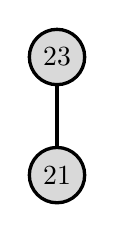
\begin{tikzpicture}[very thick,level/.style={sibling distance=60mm/#1}]
    \node [vertex] (r){$23$}{
    child {node [vertex] (a) {$21$}}
  };
  \end{tikzpicture}
\end{figure}
\begin{figure}[h]
  \centering\footnotesize
  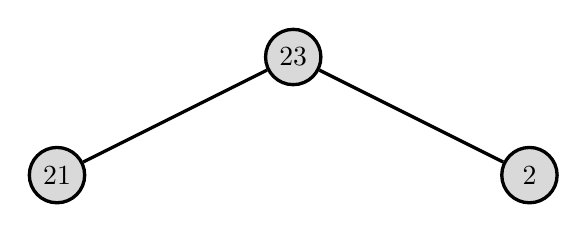
\begin{tikzpicture}[very thick,level/.style={sibling distance=60mm/#1}]
    \node [vertex] (r){$23$}{
    child {node [vertex] {$21$}}
    child {node [vertex] {$2$}}
  };
  \end{tikzpicture}
\end{figure}

\begin{figure}[h]
  \centering\footnotesize
  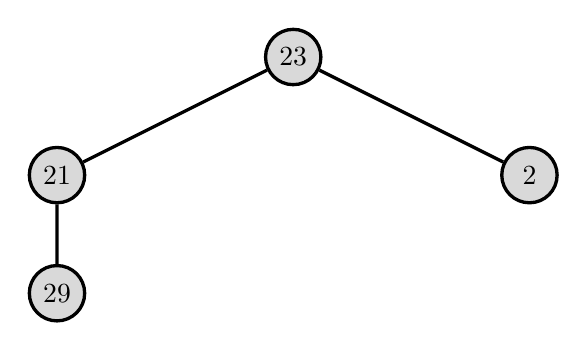
\begin{tikzpicture}[very thick,level/.style={sibling distance=60mm/#1}]
    \node [vertex] (r){$23$}{
    child {node [vertex] (a) {$21$}
    	child {node [vertex]  {$29$}}
    }
    child {node [vertex] (a) {$2$}}
  };
  \end{tikzpicture}
\end{figure}

\begin{figure}[h]
  \centering\footnotesize
  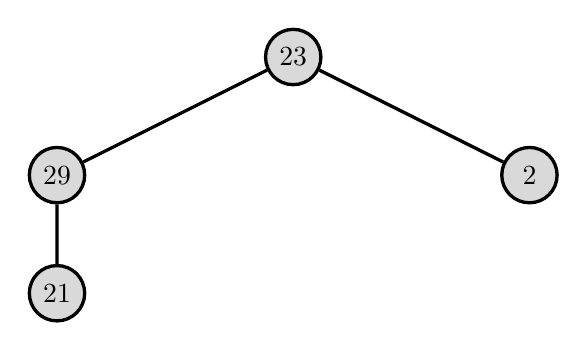
\begin{tikzpicture}[very thick,level/.style={sibling distance=60mm/#1}]
    \node [vertex] (r){$23$}{
    child {node [vertex] (a) {$29$}
    	child {node [vertex]  {$21$}}
    }
    child {node [vertex] (a) {$2$}}
  };
  \end{tikzpicture}
\end{figure}

\begin{figure}[h]
  \centering\footnotesize
  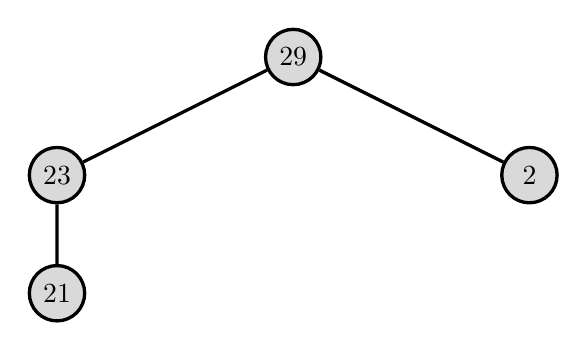
\begin{tikzpicture}[very thick,level/.style={sibling distance=60mm/#1}]
    \node [vertex] (r){$29$}{
    child {node [vertex] (a) {$23$}
    	child {node [vertex]  {$21$}}
    }
    child {node [vertex] (a) {$2$}}
  };
  \end{tikzpicture}
\end{figure}

\begin{figure}[h]
  \centering\footnotesize
  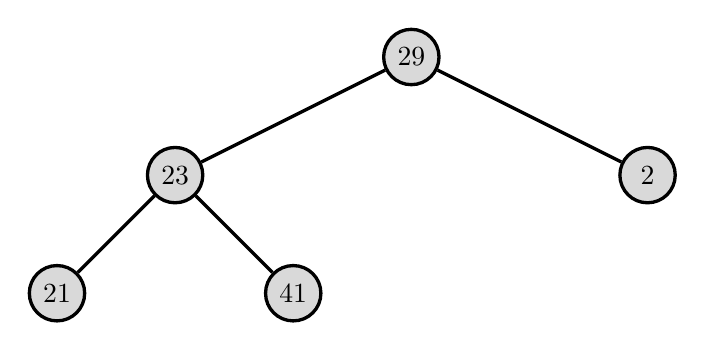
\begin{tikzpicture}[very thick,level/.style={sibling distance=60mm/#1}]
    \node [vertex] (r){$29$}{
    child {node [vertex] (a) {$23$}
    	child {node [vertex]  {$21$}}
        child {node [vertex]  {$41$}}
    }
    child {node [vertex] (a) {$2$}}
  };
  \end{tikzpicture}
\end{figure}
\begin{figure}[h]
  \centering\footnotesize
  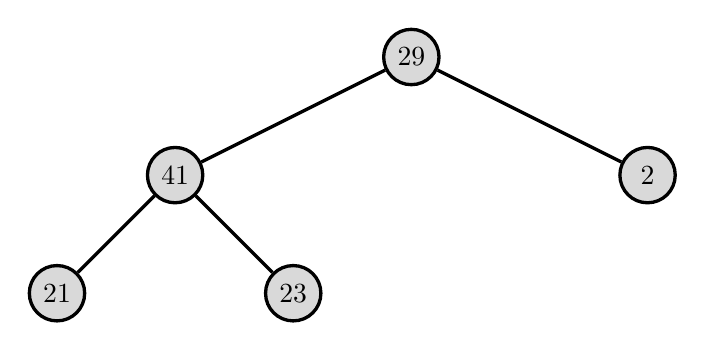
\begin{tikzpicture}[very thick,level/.style={sibling distance=60mm/#1}]
    \node [vertex] (r){$29$}{
    child {node [vertex] (a) {$41$}
    	child {node [vertex]  {$21$}}
        child {node [vertex]  {$23$}}
    }
    child {node [vertex] (a) {$2$}}
  };
  \end{tikzpicture}
\end{figure}
\begin{figure}[h]
  \centering\footnotesize
  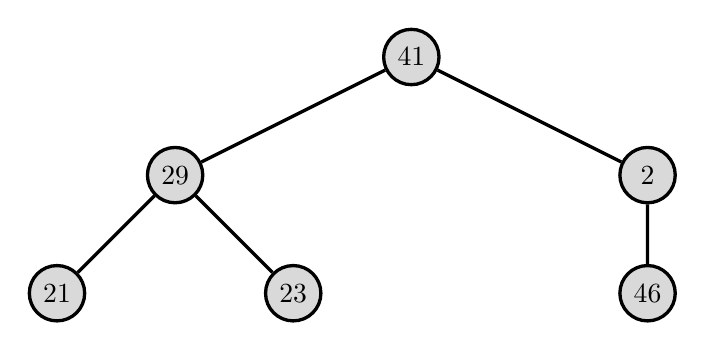
\begin{tikzpicture}[very thick,level/.style={sibling distance=60mm/#1}]
    \node [vertex] (r){$41$}{
    child {node [vertex] (a) {$29$}
    	child {node [vertex]  {$21$}}
        child {node [vertex]  {$23$}}
    }
    child {node [vertex] (a) {$2$}
		child {node [vertex] {$46$}}    
    }
  };
  \end{tikzpicture}
\end{figure}
\begin{figure}[h]
  \centering\footnotesize
  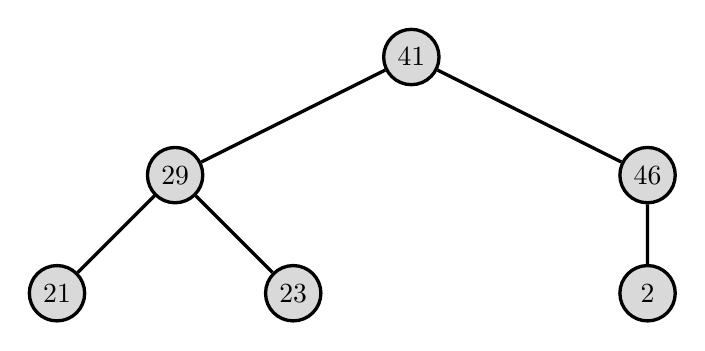
\begin{tikzpicture}[very thick,level/.style={sibling distance=60mm/#1}]
    \node [vertex] (r){$41$}{
    child {node [vertex] (a) {$29$}
    	child {node [vertex]  {$21$}}
        child {node [vertex]  {$23$}}
    }
    child {node [vertex] (a) {$46$}
		child {node [vertex] {$2$}}    
    }
  };
  \end{tikzpicture}
\end{figure}
\begin{figure}[h]
  \centering\footnotesize
  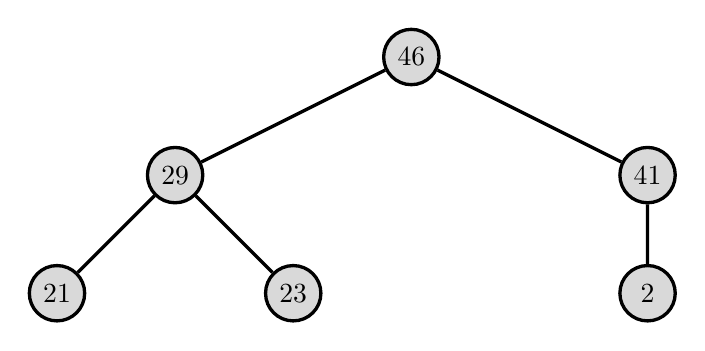
\begin{tikzpicture}[very thick,level/.style={sibling distance=60mm/#1}]
    \node [vertex] (r){$46$}{
    child {node [vertex] (a) {$29$}
    	child {node [vertex]  {$21$}}
        child {node [vertex]  {$23$}}
    }
    child {node [vertex] (a) {$41$}
		child {node [vertex] {$2$}}    
    }
  };
  \end{tikzpicture}
\end{figure}
\begin{figure}[h]
  \centering\footnotesize
  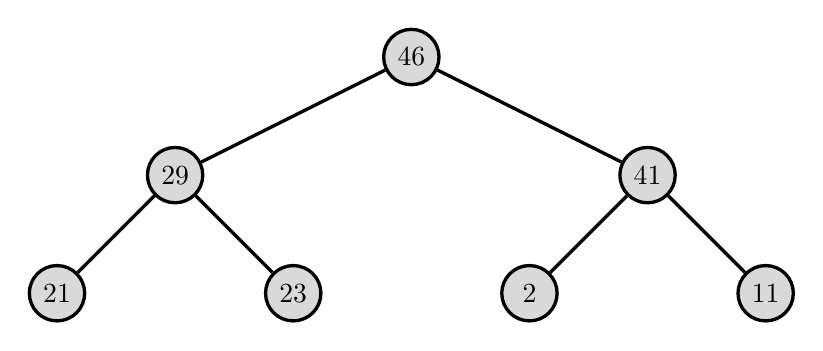
\begin{tikzpicture}[very thick,level/.style={sibling distance=60mm/#1}]
    \node [vertex] (r){$46$}{
    child {node [vertex] (a) {$29$}
    	child {node [vertex]  {$21$}}
        child {node [vertex]  {$23$}}
    }
    child {node [vertex] (a) {$41$}
		child {node [vertex] {$2$}}
        child {node [vertex] {$11$}}
    }
  };
  \end{tikzpicture}
\end{figure}
\begin{figure}[h]
  \centering\footnotesize
  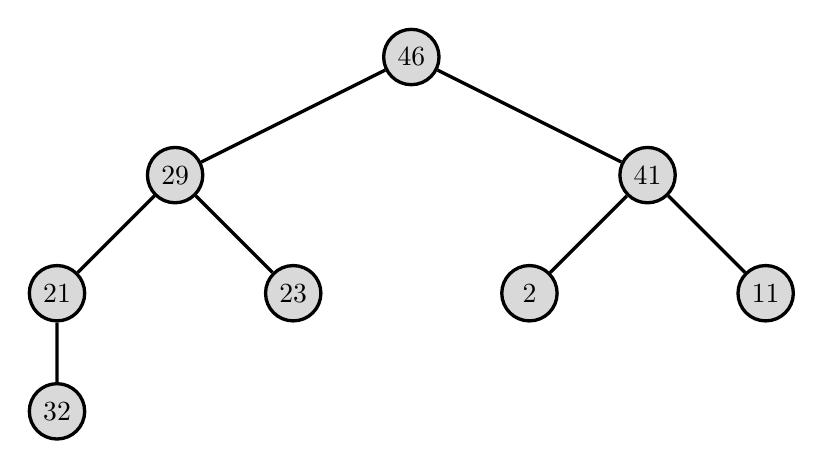
\begin{tikzpicture}[very thick,level/.style={sibling distance=60mm/#1}]
    \node [vertex] (r){$46$}{
    child {node [vertex] (a) {$29$}
    	child {
        	node [vertex] {$21$}
            child {
            	node [vertex] {$32$}
            }
        }
        child {node [vertex]  {$23$}}
    }
    child {node [vertex] (a) {$41$}
		child {node [vertex] {$2$}}
        child {node [vertex] {$11$}}
    }
  };
  \end{tikzpicture}
\end{figure}
\begin{figure}[h]
  \centering\footnotesize
  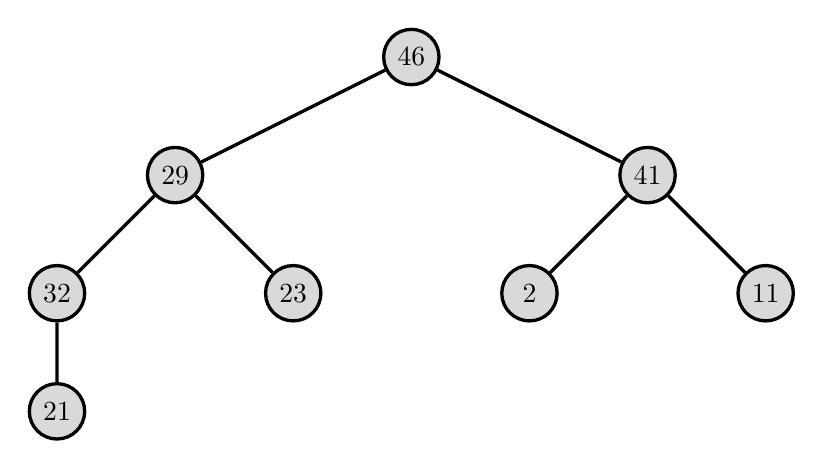
\begin{tikzpicture}[very thick,level/.style={sibling distance=60mm/#1}]
    \node [vertex] (r){$46$}{
    child {node [vertex] (a) {$29$}
    	child {
        	node [vertex] {$32$}
            child {
            	node [vertex] {$21$}
            }
        }
        child {node [vertex]  {$23$}}
    }
    child {node [vertex] (a) {$41$}
		child {node [vertex] {$2$}}
        child {node [vertex] {$11$}}
    }
  };
  \end{tikzpicture}
\end{figure}
\begin{figure}[h]
  \centering\footnotesize
  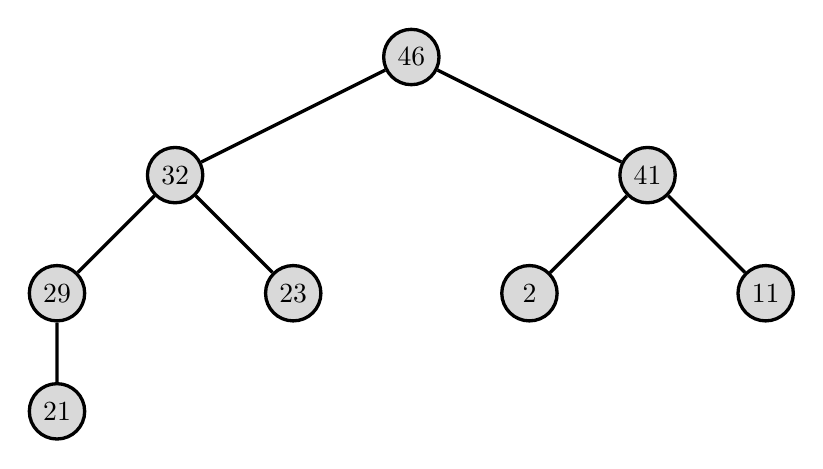
\begin{tikzpicture}[very thick,level/.style={sibling distance=60mm/#1}]
    \node [vertex] (r){$46$}{
    child {node [vertex] (a) {$32$}
    	child {
        	node [vertex] {$29$}
            child {
            	node [vertex] {$21$}
            }
        }
        child {node [vertex]  {$23$}}
    }
    child {node [vertex] (a) {$41$}
		child {node [vertex] {$2$}}
        child {node [vertex] {$11$}}
    }
  };
  \end{tikzpicture}
\end{figure}
\begin{figure}[h]
  \centering\footnotesize
  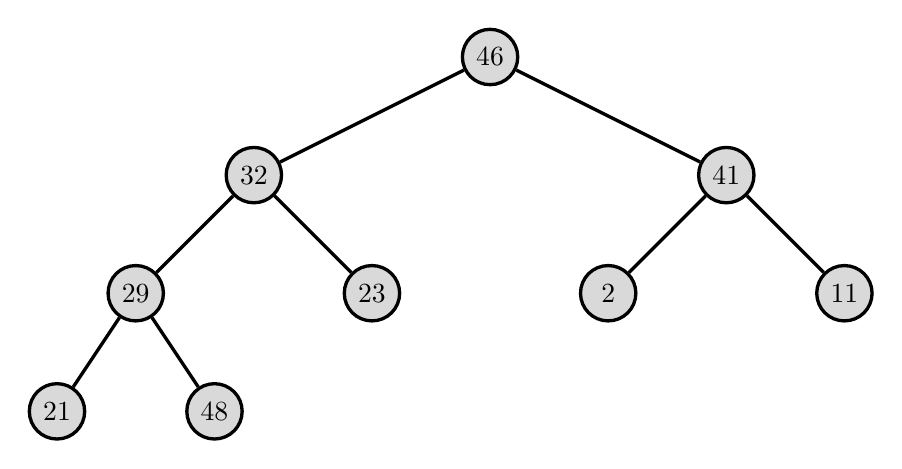
\begin{tikzpicture}[very thick,level/.style={sibling distance=60mm/#1}]
    \node [vertex] (r){$46$}{
    child {node [vertex] (a) {$32$}
    	child {
        	node [vertex] {$29$}
            child {node [vertex] {$21$}}
            child {node [vertex] {$48$}}
        }
        child {node [vertex]  {$23$}}
    }
    child {node [vertex] (a) {$41$}
		child {node [vertex] {$2$}}
        child {node [vertex] {$11$}}
    }
  };
  \end{tikzpicture}
\end{figure}
\begin{figure}[h]
  \centering\footnotesize
  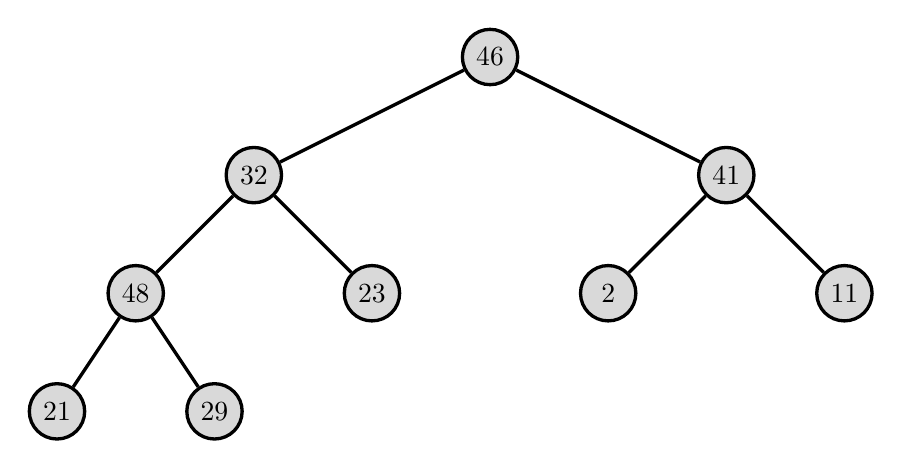
\begin{tikzpicture}[very thick,level/.style={sibling distance=60mm/#1}]
    \node [vertex] (r){$46$}{
    child {node [vertex] (a) {$32$}
    	child {
        	node [vertex] {$48$}
            child {node [vertex] {$21$}}
            child {node [vertex] {$29$}}
        }
        child {node [vertex]  {$23$}}
    }
    child {node [vertex] (a) {$41$}
		child {node [vertex] {$2$}}
        child {node [vertex] {$11$}}
    }
  };
  \end{tikzpicture}
\end{figure}

\begin{figure}[h]
  \centering\footnotesize
  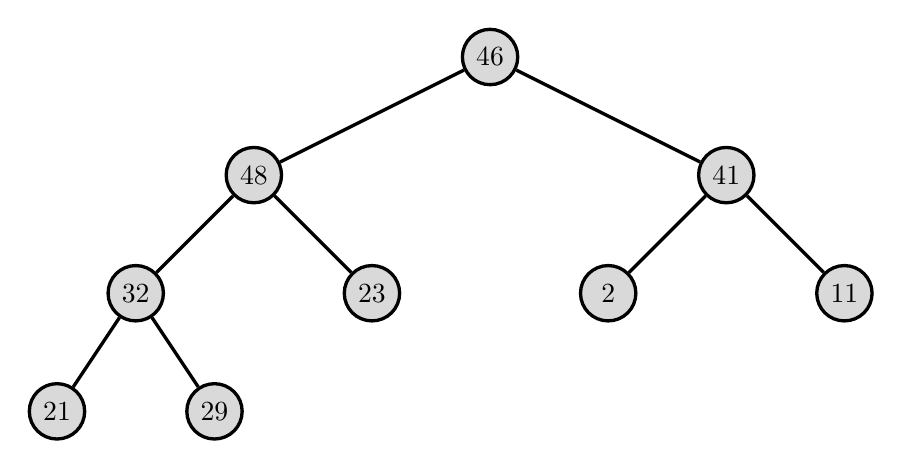
\begin{tikzpicture}[very thick,level/.style={sibling distance=60mm/#1}]
    \node [vertex] (r){$46$}{
    child {node [vertex] (a) {$48$}
    	child {
        	node [vertex] {$32$}
            child {node [vertex] {$21$}}
            child {node [vertex] {$29$}}
        }
        child {node [vertex]  {$23$}}
    }
    child {node [vertex] (a) {$41$}
		child {node [vertex] {$2$}}
        child {node [vertex] {$11$}}
    }
  };
  \end{tikzpicture}
\end{figure}
\begin{figure}[h]
  \centering\footnotesize
  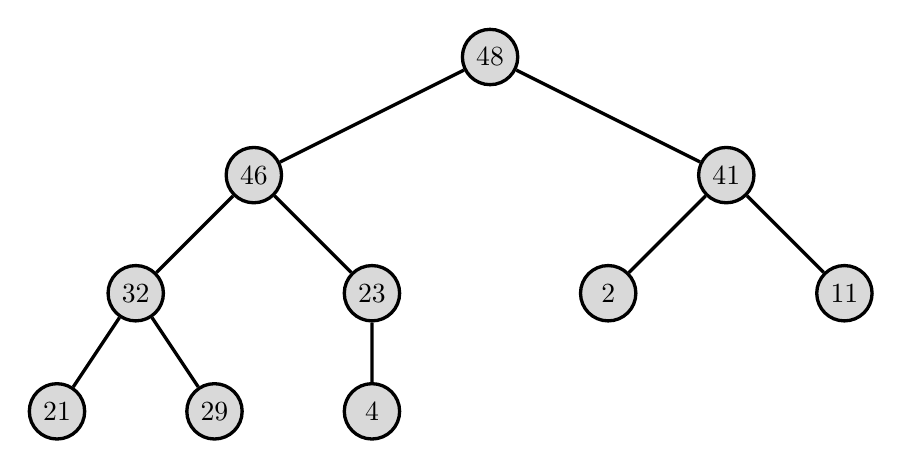
\begin{tikzpicture}[very thick,level/.style={sibling distance=60mm/#1}]
    \node [vertex] (r){$48$}{
    child {node [vertex] (a) {$46$}
    	child {
        	node [vertex] {$32$}
            child {node [vertex] {$21$}}
            child {node [vertex] {$29$}}
        }
        child {
        	node [vertex]  {$23$}
            child {node [vertex] {$4$}}
         }
    }
    child {node [vertex] (a) {$41$}
		child {node [vertex] {$2$}}
        child {node [vertex] {$11$}}
    }
  };
  \end{tikzpicture}
\end{figure}

\clearpage
\end{homeworkProblem}

%----------------------------------------------------------------------------------------
%	PROBLEM 2
%----------------------------------------------------------------------------------------

\begin{homeworkProblem}
A)\ sortA \ $32$ \
\begin{lstlisting}
// Finds the least significant bit and groups them inside a bucket.	
#define MAX_MSB_BIT 32
\end{lstlisting}
B) // SORT-B \ \ 
\begin{lstlisting}
//The number of shift operations required to make the MSB to LSB
#define BIT_SHIFT_MSB_TO_LSB 24
//The biggest int number that can be contained in an container can have the MSB at
//its 9 position. The decimal equivalent of 100000000 is 256.
#define BUCKET_MAX_SIZE 256
//In order to mask 8 bits so that any number contained more than 8 bits does not  
//generate an IndexOutOfBoundsException. More importantly, we want to consider //only the first 8 bits (from the left) and the binary representation of 255 has 8 //1s.
#define 8_BIT_MASK 255
// Sorting individual lists of elements collected in the bucket of size (i)
//It acts as a sliding window that shuts down from the MSB to LSB, where the 
// word is defined as a chunk of 8 Bits.
#define BITS_PER_WORD 8
\end{lstlisting}
\end{homeworkProblem}
\clearpage
%----------------------------------------------------------------------------------------

%----------------------------------------------------------------------------------------
%	PROBLEM 3
%----------------------------------------------------------------------------------------

% To have just one problem per page, simply put a \clearpage after each problem

\begin{homeworkProblem}
YES \\ Changing the ints to longs will make the code run for integers as large as $2^64-1$\\
\textbf{In SORT A, 32 would become 64} \\
\textbf{In SORT B, 24 would become 56} \\
\textbf{In SORT B, 256 would remain 256 }\\
\textbf{In SORT B, 255 would remain  255 } \\
\textbf{In SORT B, 8 would remain 8}\\
\end{homeworkProblem}
\clearpage
%-------------------------------------------------------------------------------
%	PROBLEM 4
%----------------------------------------------------------------------------------------

\begin{homeworkProblem}
\textbf{Best-Case Running Time}\\
\textbf{$\cdot$ SORT A} \\
\begin{lstlisting}
int n = seq.length;
int[] seq0 = new int[n];
int[] seq1 = new int[n];
int n0 = 0;                // # of items currently in seq0
\end{lstlisting}
\textbf{As the initializations take constant time}
$\Theta(1) + \Theta(1) + \Theta(1)$ \\
$\Rightarrow \ \Theta(1)$
\\
\begin{lstlisting}
for (int bitnum = 0; bitnum < 32; bitnum = bitnum + 1) {
n0 = 0;
n1 = 0;
	for (int i = 0; i < n; i = i + 1) {
		int bit = (seq[i] >> bitnum) % 2;
		if (bit == 0) {
			seq0[n0] = seq[i];
			n0 = n0 + 1;
		}
		else {
			seq1[n1] = seq[i];
			n1 = n1 + 1;
		}
	}
    .
    .
    .
}
\end{lstlisting}
\textbf{The outer for loop runs for $\Theta(32)$ times and the inner for loop runs for $\Theta(n)$ times. Thus, my fundamental theorem of arithmetic, the runtime complexity of this step is $\Theta(32\cdot n)$}

\begin{lstlisting}
	for (int i = 0; i < n0; i = i + 1) {
		seq[i] = seq0[i];
	}
	for (int i = 0; i < n1; i = i + 1) {
		seq[n0+i] = seq1[i];
	}
\end{lstlisting}
\textbf{In the best case the next two for loops will split into equal parts as $n_0$ = $n_1$ = $n/2$. The runtime complexity of this step is $2\cdot \Theta(32\cdot n/2)$}
\textbf{Adding all the terms} \\
$\Rightarrow T(n) = \Theta(32\cdot n) + 2*\Theta(32\cdot n/2)$\\
$\Rightarrow T(n) = \Theta(32\cdot n) + 2*\Theta(16\cdot n)$ \\
$\Rightarrow T(n) = \Theta(32\cdot n)$ \\
$\Rightarrow T(n) = \Theta(n)$ \\
\textbf{For some arbitary very large Bitnumber}\\
$\Rightarrow T(n,Bitnumber) = \Theta(Bitnumber\cdot n)$ \\ \\
B) SORT B
\begin{lstlisting}
	int n = seq.length;
	List<List<Integer>> lists = new ArrayList<List<Integer>>();
	for (int j = 0; j < 256; j = j + 1)
	    lists.add (new ArrayList<Integer>())
\end{lstlisting}
\textbf{The above takes $\Theta(256) \Rightarrow \Theta(1)$\\}

\begin{lstlisting}
	for (int i = 0; i < n; i = i + 1) {
	    int bits = (seq[i] >> bitnum) & 255;
	    lists.get(bits).add (seq[i]);
	}
\end{lstlisting}
\textbf{The above steps takes $\Theta(n)$ \\}

\begin{lstlisting}
for (int j = 0; j < 256; j = j + 1) {
	    int[] seqj = new int[lists.get(j).size()];
	    int k = 0;
	    for (Integer m : lists.get(j)) {
			seqj[k] = m;
			k = k + 1;
	    }
	if (bitnum > 0)
	    seqj = sortB (seqj, bitnum-8);
	for (int m : seqj) {
	    	seq[i] = m;
	   		i = i + 1;
		}
	}
\end{lstlisting}
\textbf{The best case will occur when each bin of $seq_j$(index) will contain a list of one element. Every time the sliding window shifts towards the right, the incoming word length will have one element per list. Thus, after $h$ iteration each list will have a $h$ number of elements the length of the list will equal to 256. The above step takes $\Theta(256*h) \\ \Rightarrow \ \Theta(h)$ } \\

\begin{lstlisting}
if (bitnum > 0)
	    seqj = sortB (seqj, bitnum-8)
\end{lstlisting}
\textbf{T(n,bitnumber) = T(n-8,bitnumber-8) + c \\ \\ 
Adding all the terms we have \\ \\ 
T(n,bitnumber) = T(n-8,bitnumber-8) + $\Theta(n)$\\
T(n-8,bitnumber) = T(n-16,bitnumber-16) + $\Theta(n)$
.\\
.\\
.\\
For a data-type like $long$ the number of bits required to represent a long is 64 bits. This implies that the above recurrence relation will end after 7 recurrence. For any arbitrary number of bits because of which the number of list grows $h$ high at max, the following relationship can be established -\\
$T(n-h,$ bitnumber$) = T(h, $bitnumber-h$) + min(n,h)*n$\\
T(n) = $\Theta(min(n,h))*n$ \\
For best case we shall assume that $h$ is significantly less than the n, thus $min(h,n) \Rightarrow h$ }
\textbf{The recurrence will be called 256 times in every recursion call. Thus, by Fundamental Theorem of arithmetic $256^{(24/8)+1}$}.\\ \\
\textbf{Adding all terms - } \\
$\Theta(256^{(24/8)+1}*n)$ \\
$\Rightarrow \Theta(n)$ \\ \\
\textbf{C) SORT C}
\begin{lstlisting}
	int n = seq.length;
	List<List<Integer>> lists = new ArrayList<List<Integer>>();
	for (int j = 0; j < 256; j = j + 1)
	    lists.add (new ArrayList<Integer>());
\end{lstlisting}
\textbf{The above takes $\Theta(256) \Rightarrow \Theta(1)$\\}

\begin{lstlisting}
	for (int i = 0; i < n; i = i + 1) {
	    int bits = (seq[i] >> bitnum) & 255;
	    lists.get(bits).add (seq[i]);
	}
\end{lstlisting}
\textbf{The above steps takes $\Theta(n)$ \\}

\begin{lstlisting}
	for (int j = 0; j < 256; j = j + 1) {
	    Collections.sort (lists.get(j));
	    int[] seqj = new int[lists.get(j).size()];
	    int k = 0;
	    for (Integer m : lists.get(j)) {
			seqj[k] = m;
			k = k + 1;
	    }
	    for (int m : seqj) {
			seq[i] = m;
			i = i + 1;
	    }
	}
\end{lstlisting}
\textbf{The best case will occur when Collections.sort, method needs to sort the minimum number of elements. Thus, if there is one list and all the $n$ elements are inside the one list then the runtime complexity would be $\Theta(n\cdot logn)$. However, if there are $h$ such lists, then the runtime complexity would be $\Theta(h \cdot logh)*n/h$. It is apparent that the best case would occur when all the n elements are equally divided into 256 terms \\ $h = n / 256$} \\
\\
\textbf{Adding all the terms - \\}
\textbf{T(n,bitnumber) = T(n-8,bitnumber-8) + c \\ \\ 
Adding all the terms we have \\ \\ 
T(n,bitnumber) = T(n-8,bitnumber-8) + $\Theta(h*logh)$\\
T(n-8,bitnumber) = T(n-16,bitnumber-16) + $\Theta(h*logh)$
.\\
.\\
.\\
$\Rightarrow$ T(n,bitnumber) = T(1,bitnumber-h) + $\Theta(h*logh)$\\
$\Rightarrow$ T(n,bitnumber) = $\Theta(256*(h*logh))$\\
$\Rightarrow$ T(n,bitnumber) = $\Theta(256*((n/256)*log(n/256))$\\
$\Rightarrow$ T(n,bitnumber) = $\Theta(n*log(n))$\\}
\clearpage
\end{homeworkProblem}
%Problem 5
\begin{homeworkProblem}
\textbf{Worst-Case Running Time}\\
\textbf{$\cdot$ SORT A} \\
\begin{lstlisting}
int n = seq.length;
int[] seq0 = new int[n];
int[] seq1 = new int[n];
int n0 = 0;                // # of items currently in seq0
\end{lstlisting}
\textbf{As the initializations take constant time}
$\Theta(1) + \Theta(1) + \Theta(1)$ \\
$\Rightarrow \ \Theta(1)$
\\
\begin{lstlisting}
for (int bitnum = 0; bitnum < 32; bitnum = bitnum + 1) {
n0 = 0;
n1 = 0;
	for (int i = 0; i < n; i = i + 1) {
		int bit = (seq[i] >> bitnum) % 2;
		if (bit == 0) {
			seq0[n0] = seq[i];
			n0 = n0 + 1;
		}
		else {
			seq1[n1] = seq[i];
			n1 = n1 + 1;
		}
	}
    .
    .
    .
}
\end{lstlisting}
\textbf{The outer for loop runs for $\Theta(32)$ times and the inner for loop runs for $\Theta(n)$ times. Thus, my fundamental theorem of arithmetic, the runtime complexity of this step is $\Theta(32\cdot n)$}

\begin{lstlisting}
	for (int i = 0; i < n0; i = i + 1) {
		seq[i] = seq0[i];
	}
	for (int i = 0; i < n1; i = i + 1) {
		seq[n0+i] = seq1[i];
	}
\end{lstlisting}
\textbf{In the worst case all the elements in the array will be equal and will be to the highest power of the Most Significant Bit. This will enforce the first loop to run $n$ number of times while the second loop will never run(as the aim is to maximize the runtime). The complexity of this step would be $\Theta(32*n)$\\}
\textbf{Adding all the terms} \\
$\Rightarrow T(n) = \Theta(32\cdot n) + \Theta(32\cdot n)$\\
$\Rightarrow T(n) = 2*\Theta(32\cdot n)$
$\Rightarrow T(n) = \Theta(32\cdot n)$\\
\textbf{For some arbitrary very large Bitnumber}\\
$\Rightarrow T(n,Bitnumber) = \Theta(Bitnumber\cdot n)$ \\ \\
\textbf{In our case $T(n,32) = \Theta(32\cdot n)$}\\
$T(n,32) = \Theta(n)$\\
\textbf{(B) SORT B}
\begin{lstlisting}
	int n = seq.length;
	List<List<Integer>> lists = new ArrayList<List<Integer>>();
	for (int j = 0; j < 256; j = j + 1)
	    lists.add (new ArrayList<Integer>())
\end{lstlisting}
\textbf{The above takes $\Theta(256) \Rightarrow \Theta(1)$\\}

\begin{lstlisting}
	for (int i = 0; i < n; i = i + 1) {
	    int bits = (seq[i] >> bitnum) & 255;
	    System.out.println(bits+"----");
	    lists.get(bits).add (seq[i]);
	}
\end{lstlisting}
\textbf{The above steps takes $\Theta(n)$ \\}

\begin{lstlisting}
for (int j = 0; j < 256; j = j + 1) {
	    int[] seqj = new int[lists.get(j).size()];
	    int k = 0;
	    for (Integer m : lists.get(j)) {
			seqj[k] = m;
			k = k + 1;
	    }
	if (bitnum > 0)
	    seqj = sortB (seqj, bitnum-8);
	for (int m : seqj) {
	    	seq[i] = m;
	   		i = i + 1;
		}
	}
\end{lstlisting}
\textbf{The worst case will occur when each bin of $seq_j$(index) will contain a list of all the elements. Every time the sliding window shifts towards the right, the incoming word length will have only one list and all the elements pushed to that list. Thus, after $h$ iteration each list will have a $h$ number of elements the length of the list will equal to 256. More importantly there will be $bitnum-8$ such lists of all the lists having the same element. The above step takes $\Theta(256*(bitnum-8) \\ \Rightarrow \ \Theta(h*(bitnum-8)$\\
In the worst case the algorithm will produce bitnum-8 towers of height h in total. \\ $\therefore (h*(bitnum-8) = n$ \\
$\Rightarrow \Theta(n)$} \\

\begin{lstlisting}
if (bitnum > 0)
	    seqj = sortB (seqj, bitnum-8)
\end{lstlisting}
\textbf{T(n,bitnumber) = T(n-8,bitnumber-8) + c \\ \\ 
Adding all the terms we have \\ \\ 
T(n,bitnumber) = T(n-8,bitnumber-8) + $\Theta(n)$\\
T(n-8,bitnumber) = T(n-16,bitnumber-16) + $\Theta(n)$
.\\
.\\
.\\
For a data-type like $long$ the number of bits required to represent a long is 64 bits. This implies that the above recurrence relation will end after 7 recurrence. For any arbitary number of bits because of which the number of list grows $h$ high at max, the following relationship can be established -\\
$T(n-h,$ bitnumber$) = T(h, $bitnumber-h$) + min(n,h)*n$\\
T(n) = $\Theta(min(n,h))*n$ \\}
\textbf{In our case $T(n,24) = \Theta(24\cdot n)$}
\\ $\because 24 \leq n \ ${for very large n}$.$ \\
$T(n,24) = \Theta(n)$\\ \\ \\ 
\textbf{C) SORT C}
\begin{lstlisting}
	int n = seq.length;
	List<List<Integer>> lists = new ArrayList<List<Integer>>();
	for (int j = 0; j < 256; j = j + 1)
	    lists.add (new ArrayList<Integer>());
\end{lstlisting}
\textbf{The above takes $\Theta(256) \Rightarrow \Theta(1)$\\}

\begin{lstlisting}
	for (int i = 0; i < n; i = i + 1) {
	    int bits = (seq[i] >> bitnum) & 255;
	    lists.get(bits).add (seq[i]);
	}
\end{lstlisting}
\textbf{The above steps takes $\Theta(n)$ \\}

\begin{lstlisting}
	for (int j = 0; j < 256; j = j + 1) {
	    Collections.sort (lists.get(j));
	    int[] seqj = new int[lists.get(j).size()];
	    int k = 0;
	    for (Integer m : lists.get(j)) {
			seqj[k] = m;
			k = k + 1;
	    }
	    for (int m : seqj) {
			seq[i] = m;
			i = i + 1;
	    }
	}
\end{lstlisting}
\textbf{The worst case will occur when Collections.sort, method needs to sort the maximum number of elements. Thus, if there is one list and all the $n$ elements are inside the one list then the runtime complexity would be $\Theta(n\cdot logn)$.\\}
\\
\textbf{Adding all the terms - \\}
\textbf{T(n,bitnumber) = T(n-8,bitnumber-8) + c \\ \\ 
Adding all the terms we have \\ \\ 
$\Rightarrow$ T(n,bitnumber) = $\Theta(($bitnumber$-8)*(n*logn))$\\
$\Rightarrow$ T(n,bitnumber) = $\Theta($bitnumber$*n*log(n))$\\}
\textbf{In our case \\} \\
$T(n) = \Theta (n\cdot (log(n)))$
\clearpage
\end{homeworkProblem}
%Problem 6
\begin{homeworkProblem}
\textbf{Worst Case Space Complexity}\\ \\
\textbf{$\cdot$ SORT A} \\
\begin{lstlisting}
int n = seq.length;
int[] seq0 = new int[n];
int[] seq1 = new int[n];
int n0 = 0;                // # of items currently in seq0
\end{lstlisting}
\textbf{As the initializations takes space proportional to $n$}
$\Theta(n) + \Theta(n) \\$
$\Rightarrow \ \Theta(n)$
\\
\begin{lstlisting}
for (int bitnum = 0; bitnum < 32; bitnum = bitnum + 1) {
n0 = 0;
n1 = 0;
	for (int i = 0; i < n; i = i + 1) {
		int bit = (seq[i] >> bitnum) % 2;
		if (bit == 0) {
			seq0[n0] = seq[i];
			n0 = n0 + 1;
		}
		else {
			seq1[n1] = seq[i];
			n1 = n1 + 1;
		}
	}
    .
    .
    .
}
\end{lstlisting}
\textbf{Since, the seq0 and seq1 array are reusing the space alocated to them at initialization, the above for loop takes no additional space other than scope variable initialization. $\Rightarrow \Theta(1) $\\}

\begin{lstlisting}
	for (int i = 0; i < n0; i = i + 1) {
		seq[i] = seq0[i];
	}
	for (int i = 0; i < n1; i = i + 1) {
		seq[n0+i] = seq1[i];
	}
\end{lstlisting}
\textbf{The sorted list generated by seq0 and seq1 is copied into seq. In the worst case the space occupied seq1 would be of the order of $n$. However, the space used by seq0 or seq1 will be overwritten in each loop and there is no need for any auxilary data structure to store the states.}
\textbf{Adding all the terms} \\
$\Rightarrow T(n,Bitnumber) = \Theta(n)$ \\ \\

B) SORT B
\begin{lstlisting}
	int n = seq.length;
	List<List<Integer>> lists = new ArrayList<List<Integer>>();
	for (int j = 0; j < 256; j = j + 1)
	    lists.add (new ArrayList<Integer>())
\end{lstlisting}
\textbf{The above takes $\Theta(256) \Rightarrow \Theta(1)$\\}

\begin{lstlisting}
	for (int i = 0; i < n; i = i + 1) {
	    int bits = (seq[i] >> bitnum) & 255;
	    lists.get(bits).add (seq[i]);
	}
\end{lstlisting}
\textbf{In the worst case, all the numbers will be equal. This will allow the $bits$ variable to return the same value. This will allow the $lists$ to grow linearly and the space complexity for worst case would be $\Theta(n)$ So, already $\Theta(256)$ space is allocated for the List and there will be a tower of $n$ size. So the total size will be $\Theta(256\cdot n)$ \\}

\begin{lstlisting}
for (int j = 0; j < 256; j = j + 1) {
	    int[] seqj = new int[lists.get(j).size()];
	    int k = 0;
	    for (Integer m : lists.get(j)) {
			seqj[k] = m;
			k = k + 1;
	    }
	if (bitnum > 0)
	    seqj = sortB (seqj, bitnum-8);
	for (int m : seqj) {
	    	seq[i] = m;
	   		i = i + 1;
		}
	}
\end{lstlisting}
\textbf{In the worst case there will be a seemingly large tower of n size when all the numbers present in the sequence are same or list of $n/256$ length which is possible if there 256 distinct elements which reoccur $n/256$ times. In either case the worst case space complexity would be $\Theta(256*(256*(n/256)))$ or  $\Theta(256*(1*(n)))$ \\ $\Rightarrow \ \Theta(256*n)$ } \\  $\Rightarrow \ \Theta(n)$ \\

\textbf{C) SORT C}
\begin{lstlisting}
	int n = seq.length;
	List<List<Integer>> lists = new ArrayList<List<Integer>>();
	for (int j = 0; j < 256; j = j + 1)
	    lists.add (new ArrayList<Integer>());
\end{lstlisting}
\textbf{The above takes space equivalent to $\Theta(256) \Rightarrow \Theta(1)$\\}

\begin{lstlisting}
	for (int i = 0; i < n; i = i + 1) {
	    int bits = (seq[i] >> bitnum) & 255;
	    lists.get(bits).add (seq[i]);
	}
\end{lstlisting}
\textbf{ In the worst case,when all the numbers are equal, the above steps takes $\Theta(n)$ space as all the numbers are appended in one location.\\}

\begin{lstlisting}
	for (int j = 0; j < 256; j = j + 1) {
	    Collections.sort (lists.get(j));
	    int[] seqj = new int[lists.get(j).size()];
	    int k = 0;
	    for (Integer m : lists.get(j)) {
			seqj[k] = m;
			k = k + 1;
	    }
	    for (int m : seqj) {
			seq[i] = m;
			i = i + 1;
	    }
	}
\end{lstlisting}
\textbf{As per the documentation for Collections.sort - `` dumps the specified list into an array, sorts the array, and iterates over the list resetting each element from the corresponding position in the array.`` This implies that the sorting algorithm used by Java is not in-place and this will take an additional space of $\Theta(n)$\\ It is to be noted that $\Theta(256*n) \epsilon \Theta(n)$ however, the above step will not take $\Theta(256*n)$ space as the Collections.sort() method does not allocate new space for new sort rather reuses the previous one. So, the space complexity is $\Theta(n)$ In the worst case the size of seqj would be $\Theta(n)$.
Thus, the space required for the above for loop is $2 \cdot \Theta(n)$}\\
\textbf{Adding all the terms - \\}
\textbf{Space complexity of T(n,bitnumber) = $\Theta(256*n)+2*\Theta(n)$ \\ Space complexity of T(n,bitnumber) = $\Theta(n)$}
\end{homeworkProblem}
\clearpage
\begin{homeworkProblem}
The constant factor for SORT B is $4294967296$ which is greater than than SORT A's constant factor $3$.
However,In case of SORT A we are at disadvantage as the already sorted list need to be copied again to the ``seq''. \\
The complexity of sort A $3\cdot\Theta(32*n)$ \\ 
While the complexity of SORT B $2^{12}\cdot \Theta(n)$. \\
While both the algorithms evaluates to $\Theta(n)$ Comparing both the algorithm the slope of SORT A will be greater as the $32$ is multiplied to n. 
Which for large $n$ will have a slightly higher slope than Sort B's runtime curve. This will eventually surpass the $4294967296$ constant factor.\\
$\cdot$ As the elements are randomized, there is high probability that the data will be scattered, which implies difference in the MSB's of the integers will be prominent. In that case SORT B would have better results as the terms with higher bits as 1 will be segregated from the ones with lower bits of 1. This will not be the case with SORT A as the $seq0$ will always contain elements that are not sorted and sub-array within the $seq0$ that is sorted. Thus, after every iteration we need to re-arrange the array to fit an element in the sorted sub-array\\
Therefore, I believe \textbf{SORT B} would be better.


\end{homeworkProblem}
\end{document}
